% 02_background.tex  – concise (≤ 3 pp.), details in Appendix A
% ------------------------------------------------------------------
\section{Theoretical Background \& Related Work}
\label{sec:background}

\paragraph{Notation.} We denote \(T_p\) and \(T_f\) as the numbers of observed and predicted timesteps, respectively. Following UniTraj conventions~\cite{unitrajFeng2024}, agent trajectories are represented as \(\boldsymbol{X}_d \in \R^{N_{\max} \times T_p \times F_{ap}}\) and map polylines as \(\boldsymbol{X}_s \in \R^{K_{\max} \times L \times F_{map}}\), where \(N_{\max}\) is the maximum number of agents, \(K_{\max}\) is the maximum number of map polylines, \(L\) is the points per polyline, and \(F_{ap}, F_{map}\) are the respective feature dimensions. Ground truth trajectories for the center agent are denoted \(\boldsymbol{y}_c \in \R^{T_f \times 4}\). For rasterized approaches, BEV representations use \(H \times W\) spatial resolution with \(F_d, F_s\) channel dimensions for dynamic and static inputs, respectively. Transformer models employ \(M\) output modes, \(K_s\) sampling points per deformable attention query, and \(N_h\) attention heads. Feature pyramid networks utilize \(L_{\text{FPN}}\) levels indexed by \(\ell \in \{0,\dots,L_{\text{FPN}}-1\}\), with feature maps \(C_\ell \times H_\ell \times W_\ell\) at each level. A comprehensive symbol table is provided in Appendix~\ref{app:notation}.

%--------------------------------------------------------------------

\subsection{Scene Representation Paradigms}
\label{ssec:scene_repr}

\begin{figure}[H]
\centering
\begin{subfigure}[t]{0.35\textwidth}
    \centering
    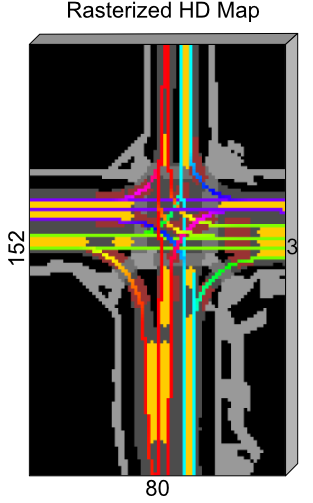
\includegraphics[width=\textwidth]{figures/caspnet-bev-repr.png}
    \caption{Rasterized BEV encoding}
    \label{fig:rasterized}
\end{subfigure}
\hfill
\begin{subfigure}[t]{0.37\textwidth}
    \centering
    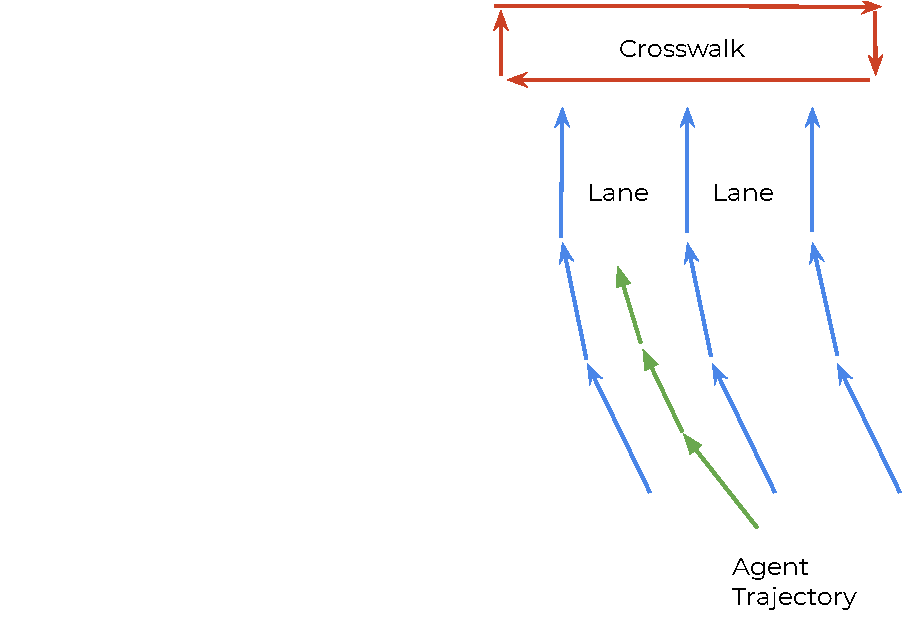
\includegraphics[width=\textwidth]{figures/vectornet-2020-vector-repr.pdf}
    \caption{Vectorized polyline preservation}
    \label{fig:vectorized}
\end{subfigure}
\caption{Scene representation paradigms in trajectory prediction: (a) rasterized approaches stack agent trajectories and HD maps into BEV images~\cite{caspnetSchäfer2022}, (b) vectorized methods preserve geometric polylines~\cite{gao2020vectornet}.}
\label{fig:scene_representations}
\end{figure}

\textbf{Raster grids.} Early systems stack past agent masks and HD-map layers into BEV images, exploiting convolutional backbones to capture local correlations while keeping runtime independent of the number of agents~\cite{cui2019multimodal,chai2019multipath}. The CASPNet family of motion forecasting models, consisting of the original CASPNet~\cite{caspnetSchäfer2022}, CASPNet++~\cite{caspnetppSchäfer2023}, and the CASPFormer~\cite{caspformerYadav2024}, exemplifies interesting architectural choices within this paradigm and will be discussed in greater detail in~\autoref{ssec:caspnet}.

\textbf{Vector tokens.} Later work encodes agents and lanes as vectorized geometric primitive such as polylines, enabling graph ( LaneGCN~\cite{liang2020learning}, VectorNet~\cite{gao2020vectornet}) or transformer based (QCNet~\cite{qcnetZhou2023}, QCNeXt~\cite{qcnextZhou2023}, LMFormer~\cite{lmformerYadav2025}) approaches with higher geometric fidelity but runtime that grows with scene complexity.\\
While only \emph{agent-centric} coordinate systems allow for tractable application of rasterized scene representations, vectorized can employ a novel paradigm to represent all coordinates in a given scene. This so-called \emph{query-centric} approach will be discussed in greater detail in~\autoref{ssec:qc_paradigm}.

% CASPNet embodies the \emph{raster} philosophy; CASPFormer adopts a hybrid strategy—retaining a CNN backbone for perception compatibility, but switching to a vectorized transformer decoder for output precision.

\subsection{The Query-Centric Paradigm}
\label{ssec:qc_paradigm}

%--------------------------------------------------------------------
\newpage